\section{Linear programming}

\subsection{Graphic example}

\begin{align*}
    f(x_1, x_2) & = 0.04 x_1 + 0.06 x_2 \\
    x_1 + x_2 & \le 10000 \\
    x_1 & \le 7500 \\
    x_2 & \le 5000 \\
    x_1, x_2 & \ge 0
\end{align*}

Let $f(x_1, x_2)$ be the function to maximize.
The feasible region, in which the variables satisfy the constraints, can be plot graphically.

\begin{figure}[H]
    \centering
    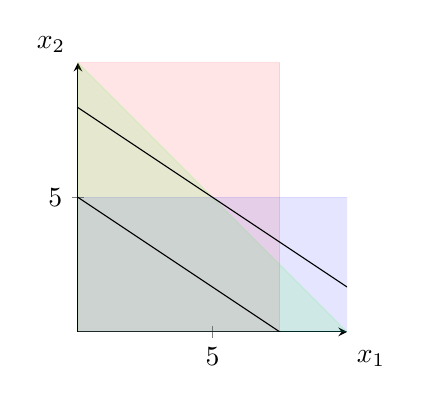
\begin{tikzpicture}
        \begin{axis}[
            axis lines=middle,
            xlabel={$x_1$},
            ylabel={$x_2$},
            xlabel style={at={(axis description cs:1,-0.1)}, anchor=west},
            ylabel style={at={(axis description cs:-0.1,1)}, anchor=south},
            xmin=0, xmax=10,
            ymin=0, ymax=10,
            xtick={5},
            ytick={5},
            domain=0:10,
            samples=10,
            width=5cm, height=5cm
        ]
        \addplot[domain=0:7.5, color=red, opacity=0.1, fill=red] {10} \closedcycle;
        \addplot[domain=0:10, color=blue, opacity=0.1, fill=blue] {5} \closedcycle;
        \addplot[domain=0:10, color=green, opacity=0.1, fill=green] {-x + 10} \closedcycle;
        \addplot[domain=0:10, color=black, opacity=1] {-x*2/3 + 5};
        \addplot[domain=0:10, color=black, opacity=1] {-x*2/3 + 25/3};
        \end{axis}
    \end{tikzpicture}
\end{figure}

In the previous chart, the black lines represent the gradient of $f(x_1, x_2) + c$.
The maximum value for $x_1$ and $x_2$ is found in the vertex of the feasible area where $c$ is at its maximum.
Solutions may be unique, if found in a vertex, multiple, if found on a feasible area side, unbounded, if the feasible is such, or infeasible if the polyhedron (feasible area) is empty (infinite number of vertices).

\subsubsection{Polyhedron vertices}

Solution are always found on a vertex, or at least on a facet, of the polyhedron.
The polyhedron is defined by the set of constraint equations: $P = \{ \ul{x} \in \mathbb{R}^n : A \ul{x} = \ul{b}, \ul{x} \ge \ul{0} \}$.
As an assumption, the matrix $A \in \mathbb{R}^{m \times n}$ is full rank, thus $m \le n$.
The facets, that are the edges found in $\mathbb{R}^2$, are obtained by setting one variable equal to zero.
The vertices are obtained by setting $n-m$ variable to zero.

\subsection{Simplex method}

The objective of the simplex method is to iter over all the vertices until an optimal solution is found.
This is done by generating a path along the edges of the polyhedron.

Some initial actions are to be taken.

Constraints that are disequalities are to be transformed into equations, by adding a slack variable.

\begin{align*}
& x_1 + x_2 \le 5 \\
& x_1 + x_2 = 5 - s_1 \\
& x_1 + x_2 + s_1 = 5
\end{align*}

A system $A \ul{x} = \ul{b}$ can be rewritten as $B \ul{x}_B + N \ul{x}_N = \ul{b}$, where $B$ is a feasible basis of $A$.

Given the problem

$$
\begin{cases}
    z = \ul{c}^T \ul{x} \\
    A \ul{x} = \ul{b}
\end{cases}
\hspace{2.5cm}
\begin{cases}
    z = - x_1 - x_2 \\
    x_1 - x_2 + s_1 = 1 \\
    x_1 + x_2 + s_2 = 3
\end{cases}
$$

where all variables are non-negative ($x_1, x_2, s_1, s_2 \ge 0$), the system can be written as

$$
A=
\begin{bmatrix}
    1 & -1 & 1 & 0 \\
    1 & 1 & 0 & 1
\end{bmatrix}
\hspace{2.5cm}
\ul{b}=
\begin{bmatrix}
    1 \\ 3
\end{bmatrix}
\hspace{2.5cm}
\ul{c}=
\begin{bmatrix}
    -1 \\ -1 \\ 0 \\ 0
\end{bmatrix}
$$

where the basis $B$ and the matrix $N$ of the partition $A = \begin{bmatrix} B N \end{bmatrix}$ are chosen to be

$$
B=
\begin{bmatrix}
    1 & 0 \\
    1 & 1
\end{bmatrix}
\hspace{2.5cm}
N=
\begin{bmatrix}
    -1 & 1 \\
    1 & 0
\end{bmatrix}
$$

making the reduced costs $\ul{c}_B$ and $\ul{c}_N$

$$
\ul{c}_B =
\begin{bmatrix}
    -1 \\ 0
\end{bmatrix}
\hspace{2.5cm}
\ul{c}_N =
\begin{bmatrix}
    -1 \\ 0
\end{bmatrix}
$$

since each of their row corresponds to the row of $\ul{c}$ equals to the $B$ and $N$ chosen columns of $A$.

From $B^{-1}$, a canonical form can be found for the previous components.

$$
\ol{\ul{c}}_N^T = \ul{c}_N^T - \ul{c}_B^T B^{-1} N
$$

$$
\ol{\ul{b}} = B^{-1} \ul{b}
$$

$$
A \ul{x} = \ul{b} \iff B \ul{x}_B + N \ul{x}_N = \ul{b} \iff x_{B_i} + \sum_{j=1}^{n-m} \ol{a}_{ij} x_{N_j} = \ol{b}_i \hspace{1em}\forall i = 1, \dots, m
$$

When moving from a vertex to an adjacent one, a column of $B$ is substituted with a column of $N$.

\subsubsection{Pivoting operation}

Given the matrix $\begin{bmatrix} \ul{b} & I \ul{s} & A \end{bmatrix}$

\begin{enumerate}
    \item select the pivot value $\ol{a}_{rs} \ne 0$,
    \item divide the $r$-th row by $\ol{a}_{rs}$,
    \item for each row $i \ne r$, subtract the resulting $r$-th row multiplied by $\ol{a}_{is}$.
\end{enumerate}

\subsubsection{Adjacent vertex}

The decision of which columns are to be switched in and out of the basis can be done via the Bland's rule.

The non basic variable to enter the basis is $s = \min\{ j : \ol{c}_j < 0 \}$ ($\ol{c}_j > 0$ for maximization problems).
The non basic variable to leave the basis is $r = \min\{ i : \ol{b}_i / \ol{a}_{is} = \theta^* \}$, where $\theta^* = \min\{b_i / a_{is} : a_{is} \ge 0\}$.

Essentially, the column $j$ of the pivot is chosen as the first where the $z$-row is negative, and the row of the pivot is the one where $b_i / a_r$ is minimal but strictly positive.

\subsubsection{Tableau algorithm}

$$
\begin{cases}
    z = - x_1 - x_2 \\
    6 x_1 + 4 x_2 + x_3 = 24 \\
    3 x_1 - 2 x_2 + x_4 = 3
\end{cases}
$$

$$
B=
\begin{bmatrix}
    1 & 0 \\
    0 & 1
\end{bmatrix}
\hspace{2.5cm}
N=
\begin{bmatrix}
    6 & 4 \\
    3 & -2
\end{bmatrix}
$$

The problem consists in finding the minimum of the objective function $z$ (maximum of $-z$).
$x_3$ and $x_4$ are the basic variables.

The first two column of the basis that have been chosen are the one of $x_3$ and $x_4$.

Firsty, build the initial tableau.

\begin{center}
    \begin{tabular}{c|c|cccc}
        & & $x_1$ & $x_2$ & $x_3$ & $x_4$ \\ \hline
        $-z$ & 0 & -1 & -1 & 0 & 0 \\ \hline
        $x_3$ & 24 & 6 & 4 & 1 & 0 \\
        $x_4$ & 6 & 3 & -2 & 0 & 1
    \end{tabular}
\end{center}

After choosing a pivot (3), exchange the row identifier ($x_4$) with the pivot column one ($x_1$), and apply the pivoting operation.

\begin{center}
    \begin{tabular}{c|c|cccc}
        & & $x_1$ & $x_2$ & $x_3$ & $x_4$ \\ \hline
        $-z$ & 2 & 0 & -5/3 & 0 & 1/3 \\ \hline
        $x_3$ & 12 & 0 & 8 & 1 & -2 \\
        $x_1$ & 2 & 1 & -2/3 & 0 & 1/3
    \end{tabular}
\end{center}

Continue until the $z$-row contains only non-negative variables.

\begin{center}
    \begin{tabular}{c|c|cccc}
        & & $x_1$ & $x_2$ & $x_3$ & $x_4$ \\ \hline
        $-z$ & 9/2 & 0 & 0 & 5/24 & -1/12 \\ \hline
        $x_2$ & 3/2 & 0 & 1 & 1/8 & -1/4 \\
        $x_1$ & 3 & 1 & 0 & 1/12 & 1/6
    \end{tabular}
\end{center}

\begin{center}
    \begin{tabular}{c|c|cccc}
        & & $x_1$ & $x_2$ & $x_3$ & $x_4$ \\ \hline
        $-z$ & 6 & 1/2 & 0 & 1/4 & 0 \\ \hline
        $x_2$ & 6 & 3/2 & 1 & 1/4 & 0 \\
        $x_4$ & 18 & 6 & 0 & 1/2 & 1
    \end{tabular}
\end{center}

Therefore, the feasible basic solution $\ul{x} = (1/2, 0, 1/4, 0)$, with $z = 6$, is optimal.

A solution may be degenerate if it contains a null basic variable.

\subsubsection{Two phase simplex method}

Since the standard simplex method starts from the vertex found in the origin, if the origin is not actually a vertex of the feasible area the algorithm won't work.

In this scenario, another iteration of the simplex method is run before hand in order to find a feasible vertex from which to start.
The first phase requires the addition of other variables $\ul{y}$ to the initial problem system, and a new objective function $v = \sum_{i=1}^m y_i$.
In particular, the system $A \ul{x} = \ul{b}$ is expanded to be $A \ul{x} + I \ul{y} = \ul{b}$.

In the following (minimization) problem the objective function is $z = x_1 + x_2 + 10 x_3$.

$$
A=
\begin{bmatrix}
    0 & 1 & 4 \\
    -2 & 1 & -6
\end{bmatrix}
\hspace{2.5cm}
\ul{b}=
\begin{bmatrix}
    2 \\ 2
\end{bmatrix}
$$

The objective function $v$ must be rewritten as a function of $\ul{x}$ variables.

\begin{align*}
& v = y_1 + y_2 \\
& y_1 = - x_2 - 4 x_3 + 2 \\
& y_2 = 2 x_1 - x_2 + 6 x_3 + 2 \\
& v = 2 x_1 - 2 x_2 + 2 x_3 + 4
\end{align*}

Therefore, here is the first phase problem to solve.

\begin{center}
    \begin{tabular}{c|c|ccc|cc}
        & & $x_1$ & $x_2$ & $x_3$ & $y_1$ & $y_2$ \\ \hline
        $-v$ & -4 & 2 & -2 & 2 & 0 & 0 \\ \hline
        $x_2$ & 2 & 0 & 1 & 4 & 1 & 0 \\
        $x_4$ & 2 & -2 & 1 & -6 & 0 & 1
    \end{tabular}
\end{center}

In the end, after a solution is found, if a $y_i$ variable is in the basis (i.e. it is the identifier of a row), it has to be swapped in with on $\ul{x}$ variable.
This is done by applying the pivoting operation with the first value of the $y_i$ row as pivot ($x_1$ column).

This is its solution.

\begin{center}
    \begin{tabular}{c|c|ccc|cc}
        & & $x_1$ & $x_2$ & $x_3$ & $y_1$ & $y_2$ \\ \hline
        $-v$ & 0 & 0 & 0 & 0 & 1 & 1 \\ \hline
        $x_2$ & 2 & 0 & 1 & 4 & 1 & 0 \\
        $x_1$ & 0 & 1 & 0 & 5 & 1/2 & -1/2
    \end{tabular}
\end{center}

Now the second phase begin.
The objective function $z$ is to be made canonical, since it should not contain the basic variable that did remain in the first phase
In this case, those basic variables are $x_2$ and $x_1$, which functions, dependent on other variables, are found from the solution system of the previous phase.

\begin{align*}
& z = x_1 + x_2 + 10 x_3 \\
& x_2 = -5 x_3 \\
& x_1 = 2 - x_3 \\
& z = 2 + 4 x_3
\end{align*}

Finally, the second phase can be started from the same table found in phase one, removing the $y$ partition and swapping in the $z$ objective function.

\begin{center}
    \begin{tabular}{c|c|ccc}
        & & $x_1$ & $x_2$ & $x_3$ \\ \hline
        $-z$ & 2 & 0 & 0 & 4 \\ \hline
        $x_2$ & 2 & 0 & 1 & 4 \\
        $x_1$ & 0 & 1 & 0 & 5
    \end{tabular}
\end{center}

On this last table (which actually already represent the best feasible solution), the simplex algorithm can be applied directly, providing $\ul{x} = (0, 0, 4)$, with $z = 2$, as best feasible solution.
